\section{Motivation} \label{sec:motivation}
Nowadays, the main stream training frameworks typically adopt the offline training
on GPPs to obtain the neural network models and then apply the quantized models to the 
target CNN accelerators. When the computing on the underlying CNN accelerators differs
from that calculated with GPPs due to the approximate arithmetic logic, overclocking or 
soft errors, the offline trained neural network models executed on the accelerator 
may deviate from the expected computing result. To evaluate the influence, 
we take Alexnet as an example and evaluate the offline trained model prediction 
accuracy on the CNN accelerators with approximate multiplier, 
overclocking, and soft errors respectively. 


  As shown in Figure 1, we adopt PipeCNN\cite{pipecnn_2} , an open sourced CNN accelerator, 
as the baseline accelerator and implement it on Xilinx KCU1500 boards. The accelerator 
runs at most 210 MHz safely for AlexNet. On a subset of ImageNet, we train AlexNet offline 
and then apply it to the accelerator. The resulting top-5 accuracy is 78.95\%. Then the clock 
frequency is boosted to 250Mhz and 260MHz respectively, we apply the original model on 
the overclocked accelerator. The performance gets improved proportionally, but the 
accuracy drops 0.5\% and 4.3\% respectively.

\begin{figure}
        \center{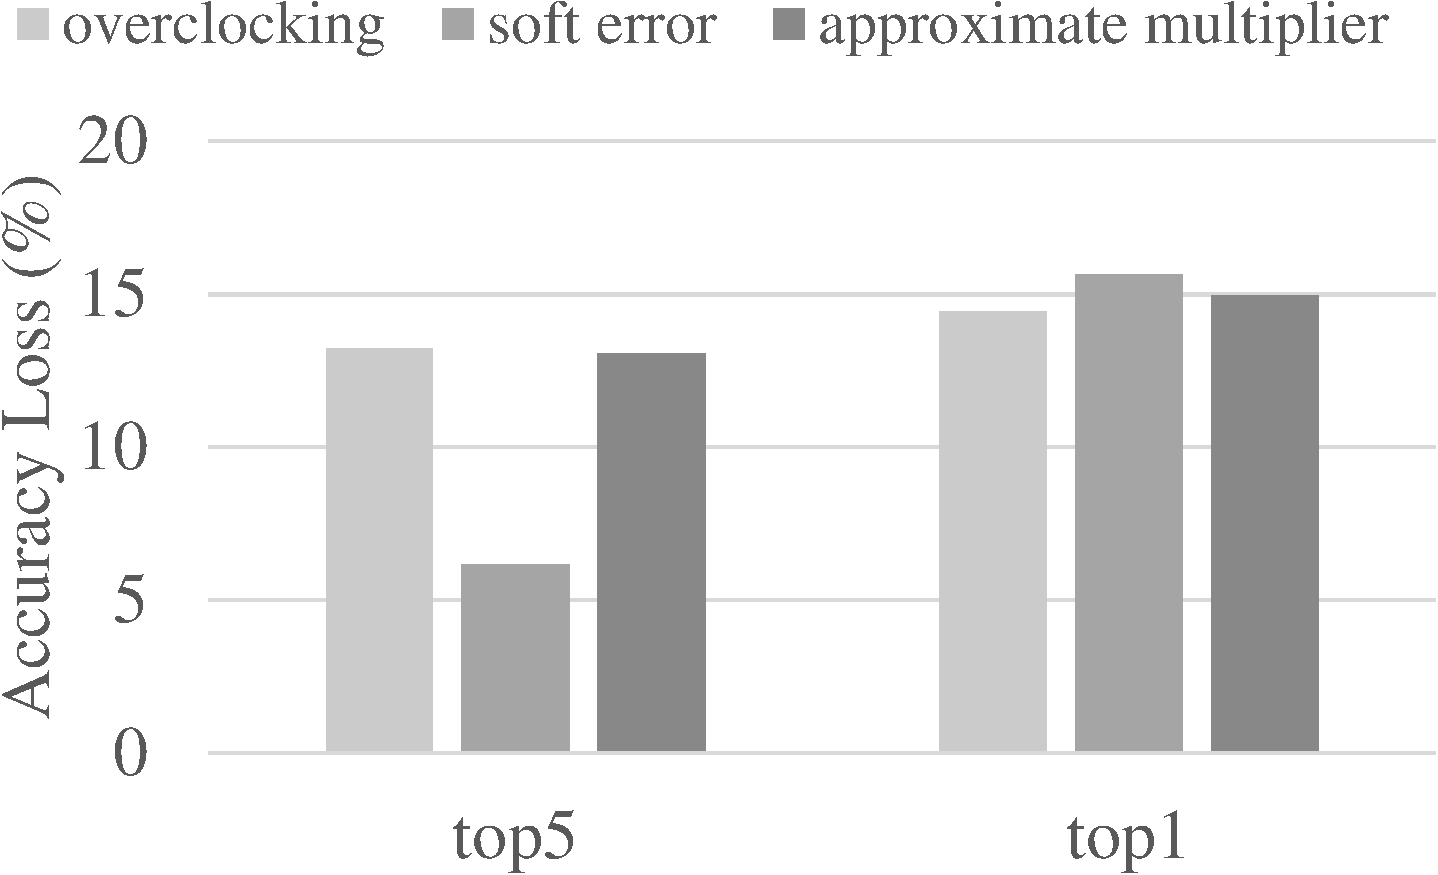
\includegraphics[width=0.85\linewidth]{accuracy_loss}}
        \caption{Influence of The CNN Accelerator’s Overclocking, Approximate multiplier and Soft error on AlexNet Model Accuracy}
        \label{fig:retrain}
%        \vspace{-0.5em}
\end{figure}

  Soft error has become an un-ignorable problem with the shrinking semiconductor 
feature size and we further analyze its influence on the CNN accelerator. 
Currently, we use a uniform distribution model to inject the SEU errors to the 
multiplication-accumulation operators (MAC) of the accelerator. It causes one-bit 
flip on random bits of the MAC results. When the error injection rate is set to 
be 0.0001\% per MAC, applying the off-line trained model to the CNN accelerator 
leads to around 0.7\% accuracy loss of the top 5 prediction. When error injection 
rate is set to be 0.001\% per MAC, the prediction accuracy drops around 3\%.

  To gain insight on the precision drop, we also check the output of the AlexNet’s last 
layer. We compare the data and find that the data deviates from expected result slightly 
due to the ‘unstable’ accelerator. But the accuracy loss of the model deployed on 
the ‘unstable’ CNN accelerator cannot be ignored according to the experiments. 
And it is highly demanded to explore the training 
system and take the accelerators’ behavior into consideration during training for higher prediction accuracy.


